\chapter{Curvature}

Given a connection on a fibre bundle, values in the bulk may be parallel transported along a curve in the base manifold.
If the curve is a closed loop, then values are not necessarily mapped back onto themselves.
The action of parallel transport around a loop known as its \textdef{holonomy}, and its deviation from the identity operator measures the connection's \emph{curvature}.

Curvature may be restated as the obstruction to the \emph{integrability} of the connection.
Therefore, the curvature of a connection may be derived by finding the integrability condition of the parallel transport equations, which is most easily done via Frobenius' theorem \cite[§6]{spivak1975dg}.

\section{Integrability and Frobenius' Theorem}
\label{sec:Frobenius}

A vector field may be \emph{integrated} by finding integral curves which are everywhere tangent to the vector field.
This notion can be generalised to higher-dimensional analogues of vector fields which associate to each point a vector \emph{subspace}, instead of merely a vector.
\begin{definition}
	A $k$-dimensional \textdef{tangent subbundle} $𝒟 ⊆ \TTℳ$ is a vector bundle $\fibrebundle[π_S] {ℝ^k} 𝒟 ℳ$ where each fibre $𝒟|_x ≅ ℝ^k$ is a $k$-dimensional subspace of $\,\TT_xℳ$.
\end{definition}
Similarly, the notion of an integral curve to a vector field may be generalised to a tangent subbundles.
\begin{definition}
	A submanifold $ℐ ⊆ ℳ$ is called an \textdef{integral manifold} of a tangent subbundle $𝒟$ if $\,\TT_xℐ \subseteq 𝒟|_x$ for all $x ∈ ℐ$.
	The subbundle $𝒟$ is called \textdef{integrable} if there exist integral manifolds through each point.
\end{definition}
For example, an integral curve of a vector field $𝒖$ through a point may be viewed as the $1$-dimensional integral manifold of the $1$-dimensional tangent subbundle described by $𝒖$.
In higher dimensions, any embedded submanifold is a maximal integral manifold of its own tangent space, viewed as a tangent subbundle in the ambient space.


An integral manifold is \textdef{maximal} if $\TT_xℐ = 𝒟|_x$, meaning the manifold dimension of $ℐ$ is the dimension of $𝒟$.
Indeed, any tangent subbundle admits $1$-dimensional integral curves, but is not maximally integrable in general.
% The integrability condition for maximal integral manifolds to exist is given by Frobenius' theorem.
The existence of maximal integral surfaces requires a special property known as \emph{involutivity}.
\begin{definition}
	A tangent subbundle $𝒟$ is \textdef{involutive} if $[𝒟, 𝒟] ⊆ 𝒟$.
	That is, if for any two sections $𝒖, 𝒗 ∈ \secs(𝒟)$ in the subbundle, their Lie bracket $[𝒖, 𝒗] ∈ \secs(𝒟)$ also lies in the subbundle.
\end{definition}
The importance of involutivity as the integrability condition for a tangent subbundle is the content of Frobenius' theorem:
\begin{theorem}[Frobenius’]
	\label{thm:Frobenius}
	If $𝒟$ is a tangent subbundle, then
	\begin{align}
		\text{$𝒟$ is integrable}
		\quad ⟺ \quad
		\text{$𝒟$ is involutive}
	.\end{align}
\end{theorem}
Frobenius’ theorem can be dualised into a statement involving exterior forms instead of vector subbundles, which can be more useful for calculation.
This stems from the observation that a vector subspace $U ⊆ V$ may be represented by the subspace $Ω$ of dual vectors with $U$ contained in their kernels,
\begin{align}
	Ω = \set{ω ∈ V^* | ω(𝒖) = 0, \forall 𝒖 ∈ U} ⊆ V^*
.\end{align}
The original subspace $U$ is recovered as $U = \bigcap_{ω ∈ Ω} \ker ω$.

\begin{definition}
	The dual representation $I$ of a tangent subbundle $𝒟$ is the ideal\,\sidenote{
		Recall from \cref{def:ideal} that an ideal (of forms) is closed under addition and satisfies $α ∧ ω ∈ I$ whenever $ω ∈ I$, for \emph{any} $α$.
	} generated by the $1$-form annihilators of $𝒟$,
	\begin{align}
		I = \gen{ω ∈ \forms[1](ℳ) | ω(𝒖) = 0, \forall 𝒖 ∈ \secs(𝒟)}
	.\end{align}
\end{definition}


The following lemma shows how the condition that $ℐ$ is an integral manifold translates between tangent subbundles and ideals.
\begin{lemma}
	Let $𝒟$ be a tangent subbundle and $I$ is its associated ideal.
	Suppose $ℐ$ is a submanifold with the inclusion map $ι : ℐ → ℳ$.
	Then,
	\begin{align}
		𝒟|_p = \TT_pℐ
		\quad ⟺ \quad
		\text{$ℐ$ is an integral manifold}
		\quad ⟺ \quad
		ι^*I = 0
	.\end{align}
\end{lemma}
\begin{proof}
	The first equivalence is by definition, included for readability.
	For the second equivalence, assume $ℐ$ is an integral manifold.
	Then, if $𝒖 ∈ \TT ℐ$ then the inclusion $\dd ι(𝒖) ∈ 𝒟$ lies in the tangent subbundle.
	Suppose $ω ∈ I$ so that $ω(𝒗) = 0$ for all $𝒗 ∈ 𝒟$.
	The restriction of $ω$ to $ℐ$ via the pullback $ι^*ω$ is identically zero, because
	\begin{align}
		(ι^*ω)(𝒖) ≡ ω\qty(\dd ι(𝒖)) = 0
	.\end{align}
	Since $𝒖$ and $ω ∈ I$ are arbitrary, we write $ι^*I = 0$.
\end{proof}
\begin{marginfigure}
	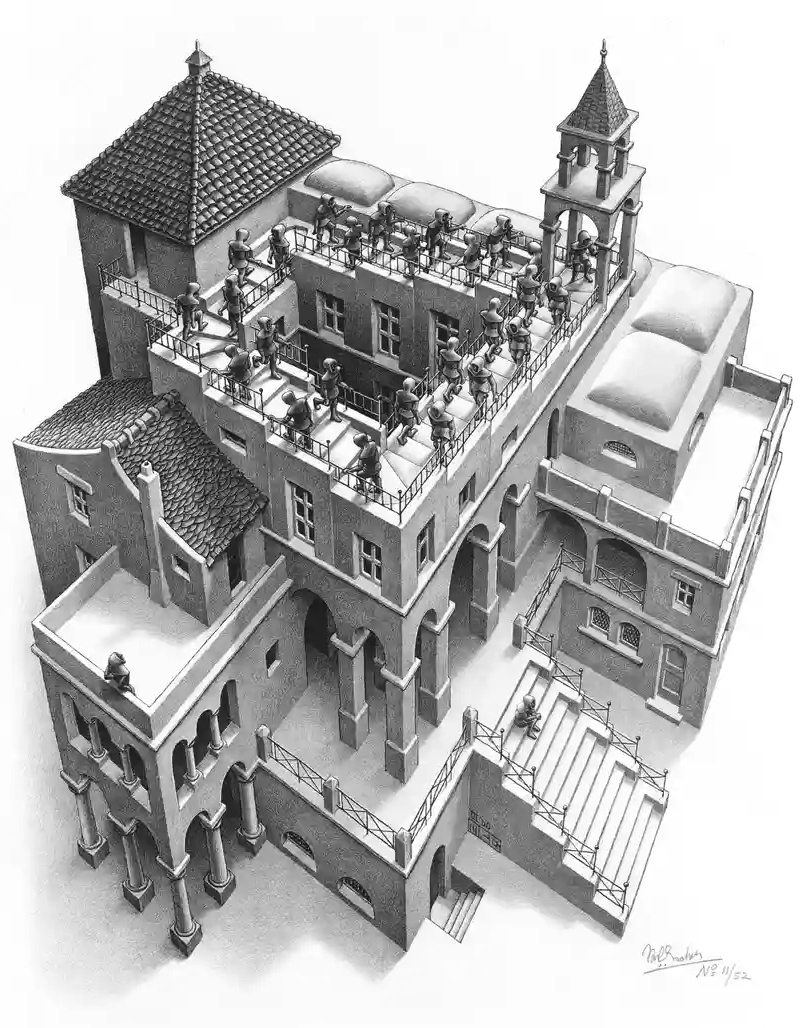
\includegraphics[width=1.05\columnwidth]{figures/penrose-stairs.png}
	\caption{
		\emph{``Ascending and Descending'' by M.\ C.\ Escher, 1960} --- perhaps the most famous illustration of an inexact $2$-form (the slope of the stairs) and its inconsistent `integral' (the impossible staircase).
	}
\end{marginfigure}
We can also translate the involutivity condition from tangent subbundles to ideals.
\begin{theorem}
	\label{thm:dual-involutive}
	If $𝒟 ⊆ \TTℳ$ is a tangent subbundle and $I ⊆ \forms[1](ℳ)$ is its associated ideal, then
	\begin{align}
		[𝒟, 𝒟] ⊆ 𝒟
		\quad ⟺ \quad
		\text{$𝒟$ is involutive}
		\quad ⟺ \quad
		\dd I ⊆ I
	.\end{align}
\end{theorem}
\begin{proof}
	The first equivalence is by definition, included for readability.
	For the second, note that the ideal $I$ is generated by $1$-forms $ω$ which vanish on $𝒟$.
	That is, $ω(𝒖) = 0$ for all $𝒖 ∈ \secs(𝒟)$, so if $𝒖, 𝒗 ∈ \secs(𝒟)$ then
	\begin{align}
		\label{eqn:xd-lb-identity}
		\dd ω(𝒖, 𝒗) &= 𝒖\qty(ω(𝒗)) - 𝒗\qty(ω(𝒖)) - ω([𝒖, 𝒗])
	\\	&= - ω([𝒖, 𝒗])
	,\end{align}
	since $ω(𝒖) = ω(𝒗) = 0$.
	If $𝒟$ is involutive then $[𝒖, 𝒗] ∈ \secs(𝒟)$ and $\dd ω(𝒖, 𝒗) = 0$.
	Thus, $\dd ω ∈ I$ if and only if $𝒟$ is involutive.
\end{proof}

Hence, by \cref{thm:Frobenius,thm:dual-involutive}, a tangent subbundle admits maximal integral surfaces if and only if its associated ideal $I$ is closed under exterior differentiation, $\dd I ⊆ I$.

Stokes’ \cref{thm:flat-stokes} states that a differential form $φ$ is integrable if it is exact (i.e., if $φ = \dd ϕ$).
On a contractible domain, this is equivalent to $φ$ being closed, by Poincaré's lemma.
In the same vein, \cref{thm:dual-involutive} states that an exterior differential system is integrable over a contractible domain if and only if its associated ideal is closed.




\subsection{Curvature as an obstruction to integrability}




We may employ Frobenius’ theorem to find the integrability condition for the connection on a vector bundle $\fibrebundle V 𝒱 ℳ$.
A linear Ehresmann connection $H$ is integrable if there exist maximal integral manifolds $f ∈ \secs(ℱ)$ which are everywhere horizontal, $\TT_p f = H_p$.
This means that $∇ f = 0$ everywhere, that parallel transport is path-independent, and that loop holonomy is always trivial.

Elaborating the condition $∇ f = 0$, we have
\begin{align}
	\label{eqn:covariantly-const}
	∇_𝒖 X = 𝒖(X) + Γ(𝒖)X = 0
	\qqtext{or}
	∂_μ X^a = -Γ_μ{}^a{}_b X^b
\end{align}
everywhere for all $𝒖 ∈ \TT ℳ$.
These equations describe the tangent subbundle $H$.
To express this, introduce coordinates $\set{x^μ}$ of $ℳ$ and linear coordinates $\set{x^a}$ of $V$ with respect to some basis.
A point $X ∈ 𝒱$ is a base point $π(X) ≡ (X^μ) ∈ ℳ$ together with a fibre value $(X^a) ∈ V$, having total coordinates
\begin{math}
	X = (X^μ, X^a)
.\end{math}
Similarly, a vector in $\TT_X 𝒱$ has components
\begin{math}
	δX = (δX^μ, δX^a)
.\end{math}

Such a vector $δX ∈ \TT_X 𝒱$ satisfies \cref{eqn:covariantly-const} if $δX^a/δX^μ = -Γ_μ{}^a{}_b X^b$, and hence the Ehresmann connection may be expressed as
\begin{align}
	\label{eqn:parallel-transport-tangent-subbundle}
	H_X = \spanof{(δX^μ, -Γ_μ{}^a{}_b X^b δX^μ) | (δX^μ) ∈ \TT_Xℳ}
\end{align}
for each $X ∈ 𝒱$.
Geometrically, this describes the change in vector components $δX^a$ induced by a nudge in the base point $δX^μ$ if $X$ is constrained to move along $H$.

To employ Frobenius’ theorem, we will find a dual representation of \cref{eqn:parallel-transport-tangent-subbundle} in terms of forms.
Any $X ∈ H$ is of the form
\begin{align}
	X = δX^μ(\∂_μ - Γ_μ{}^a{}_b X^b \∂_a)
.\end{align}
If $I$ is the ideal associated to $H$, then any $1$-form $\df ω ∈ I$ satisfies
\begin{align}
	\df ω(X) = δX^μ\qty(ω_μ - Γ_μ{}^a{}_b X^b ω_a) = 0
\end{align}
where $ω_A ≔ \df ω(\∂_A)$, implying $ω_μ =  Γ_μ{}^a{}_b X^b ω_a$ at $X$.
Written in the coordinate dual basis $\set{\df{\dd X}^μ, \df{\dd X}^a} ⊂ \TT^* 𝒱$,
\begin{align}
	\label{eqn:arbitrary-1-form-gen}
	\df ω = ω_a\qty(\df{\dd X}^a + Γ_μ{}^a{}_b X^b \df{\dd X}^μ)
\end{align}
where $ω_a$ are free scalar parameters.
Here, we adopt the notation `$\df{\phantom{ω}}$' to label differential forms for clarity.
Since \cref{eqn:arbitrary-1-form-gen} is a general $1$-form of the ideal $I$, we can see that $I$ is generated by the $1$-forms
\begin{align}
	\label{eqn:ideal-gens}
	\df Ω^a = \df{\dd X}^a + \df Γ^a{}_b X^b
,\end{align}
where we define the connection $1$-forms $\df Γ^a{}_b ≔ Γ_μ{}^a{}_b \, \df{\dd X}^μ$.

The dual formulation of Frobenius’ theorem (\cref{thm:dual-involutive}) states that the tangent subbundle $H$ is involutive if and only if the ideal $I$ is closed.
This means that $\dd \df Ω^a ∈ \dd I$ for every generator, which is equivalent to the condition $\dd\df Ω^a = \df α_a ∧ \df Ω^a$ for arbitrary `component $1$-forms' $\df α_a$.
By direct calculation,
\begin{align}
	\dd\df Ω^a &= \df{\dd^2 X^a} + \dd \df Γ^a{}_b X^b - \df Γ^a{}_b ∧ \df{\dd X^b}
\\	&= (\dd \df Γ^a{}_b + \df Γ^a{}_c ∧ \df Γ^c{}_b) X^b - \df Γ^a{}_b ∧ \df Ω^a
\end{align}
where we substitute \cref{eqn:ideal-gens} on the second line.
Therefore, $\dd\df Ω^a ∈ I$ if and only if the residual term, called the \textdef{connection $2$-form}
\begin{align}
	\label{eqn:curvature-2-form}
	\df R^a{}_b ≔ \dd \df Γ^a{}_b + \df Γ^a{}_c ∧ \df Γ^c{}_b
,\end{align}
vanishes.
These $\df R^a{}_b$ measure the obstruction to integrability of the covariant derivative, and are identified as the primary object describing the connection's curvature.



\section{Stokes' Theorem for Curvature 2-forms}

Another way of showing that parallel transport is path-independent if and only if the curvature \eqref{eqn:curvature-2-form} vanishes is by relating the holonomy of a loop to the curvature across a surface bounded by the loop.

% This is done by deriving a Stokes-like theorem for the special case of a connection $1$-form, using a
% \begin{align}
% 	\text{``} \int_Σ \df R = \oint_{∂Σ} \df Γ \text{''}
% \end{align}


\subsection{Path-ordered exponentiation}

An initial value problem of the form
\begin{align}
	\label{eqn:path-ordered-exp-ode}
	\dv{U(t)}{t} = A(t)U(t)
\end{align}
with $U(0)$ given has the solution
\begin{align}
	U(t) = e^{\int_0^t dτ A(τ)} \, U(0)
\end{align}
provided that $A(t)$ commutes with itself at all other times, $[A(t), A(s)] = 0$.
If $A(t)$ is not necessarily commutative, then the solution may still be written formally in the following way.

By a first-order Taylor expansion, the value after an infinitesimal time-step $dt$ step is
\begin{align}
	U(dt) = U(0) + ∂_tU(0)dt = (1 + A(0)dt)U(0) = e^{A(0)dt} \, U(0)
.\end{align}
The value at a finite time $t$ is then recovered by composing steps as above, forming the \textdef{path-ordered exponential}
\begin{align}
	\label{eqn:path-ordrered-exp-solution}
	U(t)U^{-1}(0) = \Pexpl[τ]\int_0^t dτ A(τ) ≔ \lim_{dt → 0} \prod_{t_i}^{t←0} e^{A(t_i)dt}
,\end{align}
where the product $\prod_{t_i}^{t←0}$ is over values $t ≥ t_i ≥ 0$ in steps of $dt$ where each exponential factor appears \emph{right-to-left} in order of increasing $t_i$.



From the observation that $∂_t(U(t)U^{-1}(t)) = 0$ we obtain the `inverse' of the original differential equation,
\begin{align}
	\label{eqn:path-ordered-exp-ode-inv}
	∂_tU(t)^{-1} = -U(t)^{-1}A(t)
,\end{align}
which is identical to \eqref{eqn:path-ordered-exp-ode} only transposed and substituting $U(t)^T \mapsto U(t)^{-1}$ and $A(t)^T \mapsto -A(t)$.
Hence, \eqref{eqn:path-ordered-exp-ode-inv} has solution
\begin{align}
	U(t)^{-1} &= U(0)^{-1}\Pexpr[τ]\int_0^t dτ (-A(τ))
\\	&= U(0)^{-1}\Pexpl[τ]\int_t^0 dτ A(τ)
.\end{align}
Hence, the left-to-right ordered exponential $\Pexpr$ is the same as a right-to-left $\Pexpl$ if the endpoints $0 ↔ t$ are swapped and the integrand $dτ \mapsto -dτ$ flips sign.

\subsubsection{The transport operator as a path-ordered exponential}

The transport operator satisfies the differential equation \eqref{eqn:trans-ode}, which for a linear connection is of the form \eqref{eqn:path-ordered-exp-ode}.
Therefore, using the initial data $\trans_{γ(0 ← 0)} = \op{id}$, \cref{eqn:trans-ode} may be solved explicitly by
\begin{align}
	\label{eqn:trans-pexp}
	\trans_{γ(s ← 0)} = \Pexpl\int_γ (-\df Γ) = \Pexpr\int_s^0 ds \, \df Γ_{\vb{\dot γ(s)}}
.\end{align}
% \Cref{eqn:trans-pexp} is the solution to \cref{eqn:trans-ode} along $γ$ with the initial data $\trans_{γ(0 ← 0)} = \op{id}$.



\subsection{Surface-ordered exponentiation}




\begin{theorem}[Stokes theorem for curvature $2$-forms]
	\label{thm:nast}
	Let $γ : [0, 1] → ℳ$ be a contractable loop with start and end point $p$.
	Let $h_λ$ be a contraction homotopy with $λ ∈ [0, 1]$ so that $h_0(x) = p$ and $h_1(x) = x$.
	Define $ξ(λ, s) ≔ h_λ(γ(s))$ as the surface swept out by $γ$ under the contraction.
	
	\begin{marginfigure}
		\includefigure[1.1\columnwidth]{homotopy}
		\caption{
			The curve $γ$ and the surface of homotopy $ξ$.
			The bold curve represents the portion of $h_λ \circ γ$ from parameter value $0$ to $s$.
		}
	\end{marginfigure}

	Let $\df Γ$ be a connection $1$-form and let $U(λ, s) ≔ \trans_{ξ(λ, s ← 0)}$ be the group element resulting from parallel transport along the path $ξ(λ, s ← 0)$.
	Then,
	\begin{align}
		\trans_{γ}
		&= \Pexpl[s]\int_γ (-\df Γ )
	\\	&= \Pexpr[λ]\int_0^1 dλ \int_0^1 ds \; U^{-1} \, \df R(∂_s ξ, ∂_λ ξ) \, U
	,\end{align}
	where $\df R = \dd\df Γ + \df Γ ∧ \df Γ$ is the curvature $2$-form.
	Note that $U ≡ U(λ, s)$ and $ξ ≡ ξ(λ, s)$.

	\toself{This awkwardly uses different path orderings. Bralić's is left-to-right.}
\end{theorem}

\begin{proof}
	Define the abbreviations
	\begin{align}
		Γ_λ &≔ \df Γ(∂_λ ξ)
	&	&\text{and}
	&	Γ_s &≔ \df Γ(∂_s ξ)
		\label{eqn:nast-working-shorthand}
	,\end{align}
	noting that $λ$ and $s$ are \emph{not} indices.
	In full component form, these would be written, e.g.,
	\begin{align}
		(Γ_λ)^a{}_b \, |_{ξ(λ, s)} = Γ_μ{}^a{}_b \, |_{ξ(λ, s)} \pdv{ξ^μ(λ, s)}{λ}
	.\end{align}
	From \cref{lem:dtrans-is-hlift}, we have
	\begin{align}
		\eval{\pdv{U(λ, s)}{s}}_{s = 0} = \dv{s} \eval{\trans_{ξ(λ, s ← 0)}}_{s = 0} = - \df Γ(∂_s ξ)
	\end{align}
	where $ξ ≡ ξ(λ, s)$, which implies
	\begin{align}
		∂_s U &= -Γ_s \, U
	&	&\text{and}
	&	∂_s U^{-1} &= U^{-1}Γ_s
	\end{align}
	where $U ≡ U(λ, s)$.
	From these two relations it follows easily that
	\begin{align}
		\label{eqn:nast-working.1}
		∂_s\qty(U^{-1}∂_λ U)
	&=	U^{-1}\qty(Γ_s ∂_λ U + ∂_λ∂_sU)
	=	-U^{-1} (∂_λ Γ_s) \, U
	\\\qqtext{and}	∂_s(U^{-1}Γ_λU)
	&=	U^{-1}(Γ_sΓ_λ + ∂_sΓ_λ - Γ_λΓ_s)U
	.\end{align}
	The sum of the two equations above is
	\begin{align}
		∂_s(U^{-1}(∂_λ + Γ_λ)U) = U^{-1}(∂_s Γ_λ + Γ_s Γ_λ - (s ↔︎ λ)) \, U
	.\end{align}
	Note that
	\begin{math}
		∂_s Γ_λ = ∂_s(Γ_μ(∂_λ ξ)) = (∂_s Γ_μ) ∂_μ ξ^μ + Γ_μ \, ∂_s∂_λ ξ^μ
	\end{math}
	and similarly for $∂_λ Γ_s$, so that mixed partial derivatives cancel, leaving
	\begin{align}
		∂_s Γ_λ - ∂_λ Γ_s = (∂_s \df Γ)(∂_λ ξ) - (∂_λ \df Γ)(∂_s ξ)
	.\end{align}
	Putting this together, we have
	\begin{align}
		∂_s(U^{-1}(∂_λ + Γ_λ)U)
		&= U^{-1} \qty((∂_s \df Γ)(∂_λ ξ) + \df Γ(∂_s ξ)\df Γ(∂_λ ξ) - (s ↔︎ λ)) \, U
	\\	&= U^{-1} (\dd\df Γ + \df Γ ∧ \df Γ)(∂_s ξ, ∂_λ ξ) \, U
	\\	&= U^{-1} \df R(∂_s ξ, ∂_λ ξ) \, U
		\label{eqn:nast-working.2}
	.\end{align}

	Recall that $U$ and $U^{-1}$ are the group elements which parallel transport vectors along $ξ(λ, s ← 0)$ and back again, respectively.
	Also, note that $\df R$ is a $\liealg{gl}(\manif V)$-valued $2$-form, which acts to infinitesimally transform vectors in $𝒱$.
	With these in mind, it is clear that \cref{eqn:nast-working.2} is an infinitesimal linear map from the fibre $𝒱_p$ to itself.\sidenote{
		Imagine the right-hand side of \cref{eqn:nast-working.2} acting on a vector $X$.
		First, $X$ is transported by $U$ from $ξ(λ, 0) = p$ to $ξ(λ, s)$, then transformed infinitesimally by $\df R$, and finally transported back to the fibre at $p$ by $U^{-1}$.
	}
	Thus, it is well-defined to integrate \cref{eqn:nast-working.2} with respect to $s$, to obtain a finite linear transformation on $𝒱_p$.
	% We will find that this is exactly the holonomy around $h_λ γ$.

	Integrating the left-hand side of \cref{eqn:nast-working.2} yields
	\begin{align}
		\label{eqn:nast-working.3}
		\int_0^1 ds \, U^{-1}(λ, 1)(∂_λ + Γ_λ)U(λ, 1)
		= U^{-1}(λ, 1) ∂_λ U(λ, 1)
	\end{align}
	since $Γ_λ = \df Γ(∂_λ ξ(λ, s))$ vanishes at $s ∈ \set{0, 1}$ because $ξ(λ, 0) = ξ(λ, 1) = p$ is constant.
	Thus, integrating both sides yields
	\begin{align}
		U^{-1}(λ, 1) ∂_λ U(λ, 1)
		= \int_0^1 ds \, U^{-1} \df R(∂_s ξ, ∂_λ ξ) \, U
	.\end{align}
	This is an initial value problem of the form $∂_λ U(λ, 1) = U(λ, 1)A(λ)$, whose solution at $λ = 1$ may be given as the path-ordered exponential
	\begin{align}
		U(1, 1) = U(1, 0) \Pexpr\int_0^1 dλ \, A(λ)
	\end{align}
	where $A(λ)$ is the right-hand side of \cref{eqn:nast-working.3}.
	Since $U(1, 1) = \trans_γ$ and $U(1, 0) = \op{id}$, this shows the right-hand side of the theorem.
\end{proof}


\begin{corollary}
	Parallel transport is path-independent if and only if curvature vanishes everywhere.
\end{corollary}
\begin{proof}
	If the curvature vanishes everywhere, then by \cref{thm:nast} the holonomy around any loop is trivial, implying the transport operator between two fixed points is path-independent.

	Conversely, if parallel transport is path-independent, then the transport operator around any loop $γ$ is the identity.
	By \cref{thm:nast}, this implies that the total curvature on a surface bounded by $γ$ is zero.
	But since the surface and loop are arbitrary, the curvature must vanish everywhere.
\end{proof}

